\documentclass[12pt, a4paper]{article}
\usepackage[slantfont, boldfont]{xeCJK}
\usepackage{ulem}
\usepackage{amsmath}
\usepackage{booktabs}
\usepackage{colortbl}
\usepackage{amsmath}
\usepackage{algorithm}
\usepackage{algpseudocode}
\usepackage{amsmath}
\renewcommand{\algorithmicrequire}{\textbf{Input:}}  % Use Input in the format of Algorithm
\renewcommand{\algorithmicensure}{\textbf{Output:}} % Use Output in the format of Algorithm
\usepackage{indentfirst}
\usepackage[top = 1.0in, bottom = 1.0in, left = 1.0in, right = 1.0in]{geometry}
\usepackage{listings}
\usepackage{enumerate}
\usepackage{multirow}
\usepackage[usenames,dvipsnames]{xcolor}
\usepackage{graphicx}

\setCJKmainfont{SimSun}
\setCJKmonofont{SimSun}

\setlength{\parskip}{0.5\baselineskip} %行距
\setlength{\parindent}{2em} %缩进

\newcolumntype{Y}{>{\columncolor{red}}p{12pt}}
\newcolumntype{N}{>{\columncolor{white}}p{12pt}}

\renewcommand\arraystretch{1.2} %表格行高

\title{省选模拟赛-Day1}
\author{VanishD}
\begin{document}
\maketitle
\begin{tabular}{|p{90pt}|p{90pt}|p{90pt}|p{90pt}|}
	\hline
	题目名称 & 小D的奶牛 & 小D的交通 & 小D的远航 \\
	\hline
	目录 & cows & teleports & sailing \\
	\hline
	可执行文件名 & cows & teleports & sailing \\
	\hline
	输入文件名 & cows.in & teleports.in & sailing.in \\
	\hline
	输出文件名 & cows.out & teleports.out & sailing.out \\
	\hline
	每个测试点时限 & $1s$ & $1s$ & $1s$ \\
	\hline
	内存限制 & 512MB & 512MB & 512MB \\
	\hline
	试题总分 & 100 & 100 & 100 \\
	\hline
	测试点数目 & 10 & 10 & 20 \\
	\hline
	每个测试点分值 & 10 & 10 & 5 \\
	\hline
	是否有部分分 & 否 & 否 & 否 \\
	\hline
	题目类型 & 传统型 & 传统型 & 传统型 \\
    \hline
\end{tabular}

\newpage
\section{小D的奶牛}
\subsection{题目背景}
	暑假,小D去了一个神奇的岛屿度假,在这个岛上有一群有神奇的奶牛。
\subsection{题目描述}

	岛屿上的奶牛一共有$N$只,每一天,有一部分奶牛去工作,另一部分奶牛去玩乐。哪些奶牛去工作由奶牛首领决定。

	奶牛们都是暴躁老哥,一旦工作安排使他们不满就会发生暴动;具体来说如果某天去工作的奶牛中存在两只奶牛不是朋友关系,它们就会烦躁;或者某天的工作安排和之前某天相同,他们会厌倦,这两种情况下就会暴动。

	显然,暴动是一定会发生的。奶牛首领想要暴动尽量晚发生,向小D询问暴动最晚的发生时间;但小D还要忙着颓废,于是把这个问题交给了你。

\subsection{输入格式}
	
从文件cows.in中读入数据。

第一行一个整数$N$,描述奶牛的数量。

接下来$N$行,每行$N$个0/1字符描述关系矩阵$A$。

若$A_{i,j}=1$表示$i$和$j$是朋友关系。

保证$A_{i,j}=A_{j,i}$,$A_{i,i}=0$

\subsection{输出格式}

输出到文件cows.out中。

一行一个整数$Ans$,奶牛最晚发生暴动的时间。

\subsection{样例1输入}
\begin{quote}
\begin{verbatim}
3
011
101
110
\end{verbatim}
\end{quote}
\subsection{样例1输出}
\begin{quote}
\begin{verbatim}
8
\end{verbatim}
\end{quote}
\subsection{样例解释}

任何非空集合都是合法的工作集合,共$7$种。

所以最迟在第$8$天发生暴动。

\subsection{样例2输入}
\begin{quote}
\begin{verbatim}
6
011100
101100
110100
111000
000001
000010
\end{verbatim}
\end{quote}
\subsection{样例2输出}
\begin{quote}
\begin{verbatim}
19
\end{verbatim}
\end{quote}
\subsection{样例3}
	
见下发文件$cows3.in/cows3.ans$

\subsection{数据范围和约定}

对于$100\%$的数据,$N\leq 50$

详细数据范围见下表:

\begin{tabular}{|c|p{40pt}<{\centering}|c|}
	\hline
	测试点编号 & $N$ & 特殊性质\\
	\hline
	1 & $\leq 9$ & \multirow{3}{*}{无} \\
	\cline{1-2}
	2 & \multirow{2}{*}{$\leq 20$}& \\
	\cline{1-1}
	3 & & \\
	\cline{1-3}
	4 &\multirow{7}{*}{$\leq 50$} & \multirow{2}{*}{每个奶牛的朋友数量不超过20} \\
	\cline{1-1}
	5 & & \\
	\cline{1-1}\cline{3-3}
    6 & & \multirow{5}{*}{无} \\
    \cline{1-1}
    7 & &\\
    \cline{1-1}
    8 & &\\
    \cline{1-1}
    9 & & \\
    \cline{1-1}
	10 & & \\
    \hline
\end{tabular}

\newpage
\section{小D的交通}

\subsection{题目背景}

	在小D所处的岛上有一个神奇的交通运输系统,有着超出奶牛所理解的智慧。

\subsection{题目描述}

	为了解决岛屿上间的交通问题,一种转移技术应运而生,它可以快速传送物体。

	具体来说,在小岛上共有$N$个居民点,标号为$1..N$。每个居民点上都有一个转移站,为了避免混乱,并不是每对转移站都直接连通,而是遵循一定规律:

	首先,一个正数$X$被选择用来确定连通参数。
	
	接下来,对于任意两个居民点$i,j$,如果$X+i-1$与$X+j-1$的最大公约数不为$1$,则居民点$i,j$上的转移站可以直接相互连接。

	为了避免孤立,防止恐慌,一个连通参数$X$是优秀的,当且仅当按此种方式连接后,整个小岛中的每一对居民点可以通过转移站直接或间接到达(即居民点连通)。

	现在小D想考考你,一个可行的优秀的连通参数$X$是多少?

\subsection{输入格式}

	从文件teleports.in中读取数据。

	一行一个整数$N$,描述居名点的个数。

\subsection{输出格式}

	输出到文件teleports.out中。

	如果不存在一个位数小于等于100000的优秀的连通参数$X$,输出“No solution”(不包括引号)。

	否则输出任意一个优秀的连通参数$X$,不超过100000位。

\subsection{样例1输入}
\begin{quote}
\begin{verbatim}
2
\end{verbatim}
\end{quote}
\subsection{样例1输出}
\begin{quote}
\begin{verbatim}
No solution
\end{verbatim}
\end{quote}
\subsection{样例解释}

	无论$X$取多大,$X+1-1$与$X+2-1$一定互质,所以一定不连通。

\subsection{样例2输入}
\begin{quote}
\begin{verbatim}
100
\end{verbatim}
\end{quote}
\subsection{样例2输出}
\begin{quote}
\begin{verbatim}
1306976361738009591601284672880050414
\end{verbatim}
\end{quote}

\subsection{样例2解释}

	可行的解还有很多,这里只是一个例子;

\subsection{数据范围和约定}

	对于$10\%$的数据:$N \leq 15$;

	对于$30\%$的数据:$N \leq 40$;
	
	对于$50\%$的数据:$N \leq 200$;

	对于$100\%$的数据,$1 \leq N \leq 100000$。

\newpage
\section{小D的远航}
\subsection{题目背景}

	为了在奶牛的暴动前离开这座岛屿,小D造好了一艘船准备远航。

\subsection{题目描述}

	作为一个老司机兼强迫症患者,小D造的船严格满足很多规则:它有一个对称轴和一个合适的形状:可以把这个轴看做船的中轴,船的船头、船尾很窄,逐渐向船的内部变宽。(换句话说,在中轴上存在一个不一定是中点的点,从它向船的两侧宽度单调不增)。小D喜欢整数,因此船的对称轴一定位于整点处。

	不幸的是,小D的船停在一个充满礁石的内海,地形非常险恶;同时,小D的船非常不灵活,只能向上下左右四个方向航行,且不能转向。

	为了驶离内海,小D绘制了岛屿的地形图,地形图上标记了障碍、水面和船的当前位置,在航行的过程中,船的任何部位不能碰到障碍(可以相邻)。

	在内海上航行非常艰难,小D想要尽快驶离内海,因此,他想请你算出驶离内海的最短航程。

	内海外面就是海洋,所以可以认为地形图之外的位置都是可以航行的。

	船离开了内海,当且仅当船的任何一部分都不在地形图上。

\begin{quote}
\begin{verbatim}
..................................................................
..........................r.......................................
...rrr.........r........rrrrr........rrr..........................
..rrrrr.....rrrrrr......rrrrr.......rrrrrrr........rrrrrr.........
...rrr.........r........rrrrr..........rrr.........rrrrrr.........
.........................rrr......................................
..........................r.......................................
..................................................................
..................................................................
\end{verbatim}
\end{quote}
以上前三个是一艘船(第三个是竖着的),后两个不是(第5个没有整点对称轴)。

\subsection{输入格式}

	从文件sailing.in中读入数据。

	第一行一个整数$N$描述地图的大小。

	接下来$N$行,每行$N$个字符描述矩阵$A$,表示地形。
	
	$A_{i,j}='X'$表示这一格是障碍。

	$A_{i,j}='.'$表示水面。

	$A_{i,j}='r'$表示这一格是船的一部分。

	保证所有的$'r'$互相连通,且满足题目中船的性质。

\subsection{输出格式}

	输出到文件sailing.out中	

	如果船可以完全离开这片海域,输出离开海域的最小步数,否则输出"NIE"。

\subsection{样例1输入}
\begin{quote}
\begin{verbatim}
10
..........
..........
..r.......
.rrrX.....
rrrrr.....
.rrr......
X.r.......
.Xr.......
..........
..........
\end{verbatim}
\end{quote}
\subsection{样例1输出}
\begin{quote}
\begin{verbatim}
10
\end{verbatim}
\end{quote}
\subsection{样例解释}
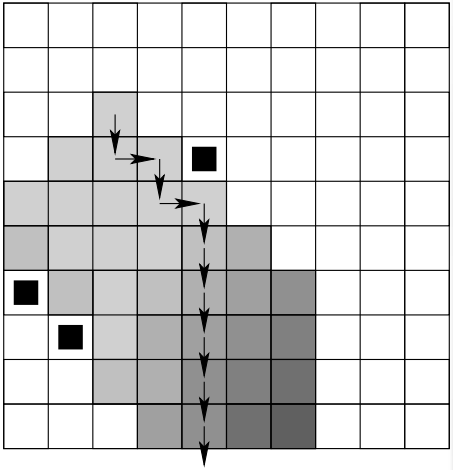
\includegraphics[scale=0.5]{sailing.png}
\subsection{样例2输入}
\begin{quote}
\begin{verbatim}
25
X..XXXXXXXXXXXXXX........
X.XXXXXXXXXXXXXXX.X..X...
X.X........r....X..X..X..
X.X........rr...X...X.X..
X.X........rrr..X..X.....
X.X........rrrr.X........
X.X....rrrrrrrrrX.....X..
XX.........rrrrX.X..X....
X..........rrrX..........
XX.........rrX...........
X..........rX............
XX.........X.............
XX.......................
X........................
XX.......................
X........................
XX.......................
XX...................X...
XX.......................
X....................X...
X........................
XXXX..XXXX...........X...
XXXX...XXXX..............
.XXX...X.X.X.....X.X.X...
X.X.X.XXXXXX.X..X....X.X.
\end{verbatim}
\end{quote}
\subsection{样例2输出}
\begin{quote}
\begin{verbatim}
42
\end{verbatim}
\end{quote}
\subsection{样例3}
	
见下发文件$sailing3.in/sailing3.ans$

\subsection{数据范围和约定}
\begin{tabular}{|c|p{40pt}<{\centering}|c|}
	\hline
	测试点编号 & $N$ & 特殊性质\\
	\hline
	1 & $\leq 100$ & \multirow{4}{*}{无} \\
	\cline{1-2}
	2 & \multirow{3}{*}{$\leq 400$}& \\
	\cline{1-1}
	3 & & \\
	\cline{1-1}
	4 & & \\
	\cline{1-3}
	5 & \multirow{16}{*}{$\leq 2000$}& \multirow{2}{*}{保证船的形状是平行于坐标轴的矩形} \\
	\cline{1-1}
	6 & & \\
	\cline{1-1}\cline{3-3}
	7 & & \multirow{2}{*}{保证船的形状是与坐标轴成45°角的正方形} \\
	\cline{1-1}
    8 & & \\
    \cline{1-1}\cline{3-3}
    9 & & \multirow{4}{*}{数据类似真实的水路地图,海岸线较为平缓}\\
    \cline{1-1}
    10 & & \\
    \cline{1-1}
    11 & & \\
    \cline{1-1}
	12 & & \\
	\cline{1-1}\cline{3-3}
	13 & & \\
	\cline{1-1}
	14 & & \\
	\cline{1-1}
	15 & & \\
	\cline{1-1}
	16 & & \\
	\cline{1-1}
	17 & & \\
	\cline{1-1}
	18 & & \\
	\cline{1-1}
	19 & & \\
	\cline{1-1}
	20 & & \\
    \hline
\end{tabular}

\end{document}